\section{Разработка и внедрение в эксплуатацию}

\subsection{Предобработка и первичный анализ данных}

Используемые данные были собраны из базы данных ClickHouse.
Период собранных данных: от 2 февраля по 11 июня 2020 года.
Данные представляют собой набор около миллиона строк в JSON формате,
которые имеют следующие признаки:

\begin{itemize}
    \item состояние (state) -- категориальный признак, отображающий состояние станка;
    \item оператор станка (operator) -- ФИО оператора станка, выполняющего работы в момент $t$;
    \item название программы (program) -- название запущенной программы;
    \item режим работы лазера (mode), например, автоматический или ручной;
    \item ампераж (amperage);
    \item вольтаж (voltage);
    \item счетчик металлических листов (sheet counter);
    \item температура лазера;
    \item мощность лазера;
    \item установленная мощность лазера;
    \item время в Unix формате.
\end{itemize}

Основными анализируемыми параметрами являются: время,
мощность и температура лазера, установленная мощность лазера.
На момент сбора данных не было возможности
собирать данные по вольтажу и амперажу,
поэтому значения в этих параметров нулевые.
Также не было возможности взятия статистики
по ошибкам программ, так как все ошибки записывались
в связи с запущенными программами.
Данные проблемы будут решены в последующих разработках.

\subsubsection{Проверка на нормальность}

Первым этапом анализа была проверка распределений,
генерируемых временные ряды, на близость к нормальному.
Для этого использовался K-квадрат тест д'Агостина,
который позволяет определить меру сходимости исходого распределения к нормальному.
Гипотеза $H_0$ заключалась в том, что заданное распределение не является нормальным.
Для этого использовалась оценка p-значения.

\begin{figure}[H]
    \center{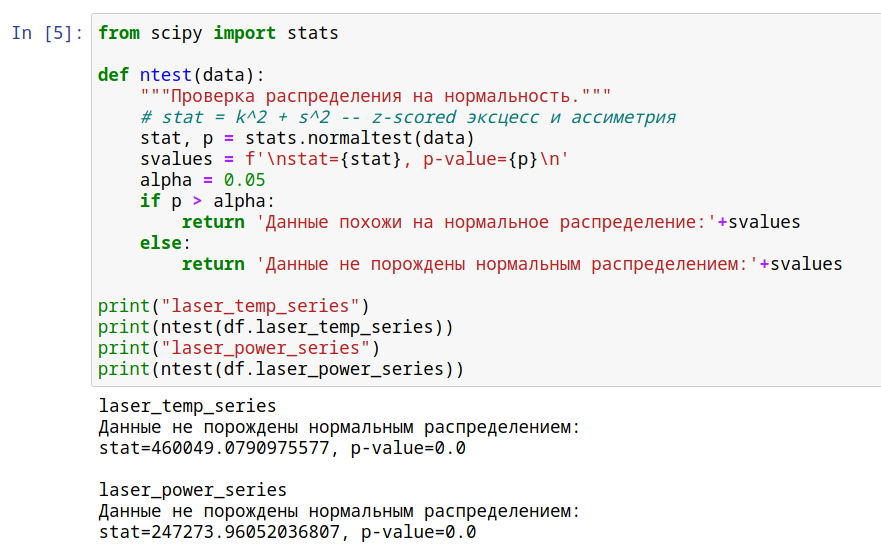
\includegraphics[width=14cm]{normaltest.png}}
    \caption{Тестирование распределений температуры и мощности лазера}
    \label{normaltest}
\end{figure}

Из рисунка \ref{normaltest} видно, что распределения температуры и мощности
не имеют нормальную структуру.

Для более точного представления структуры данных
были вычислены коэффициенты эксцесса и асимметрии.

\begin{figure}[H]
    \center{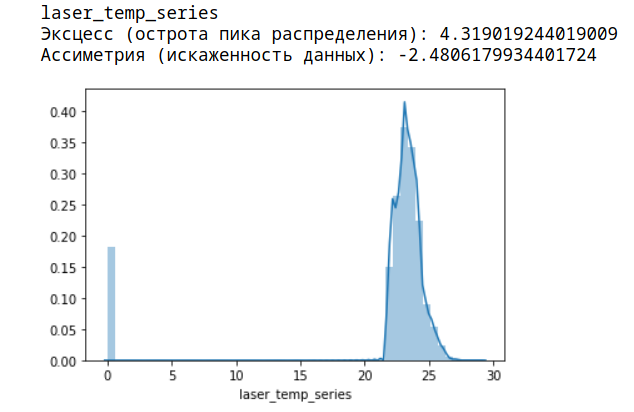
\includegraphics[width=13cm]{tempstruct.png}}
    \caption{Проверка структуры распределения температуры лазера}
    \label{tempstruct}
\end{figure}

\begin{figure}[H]
    \center{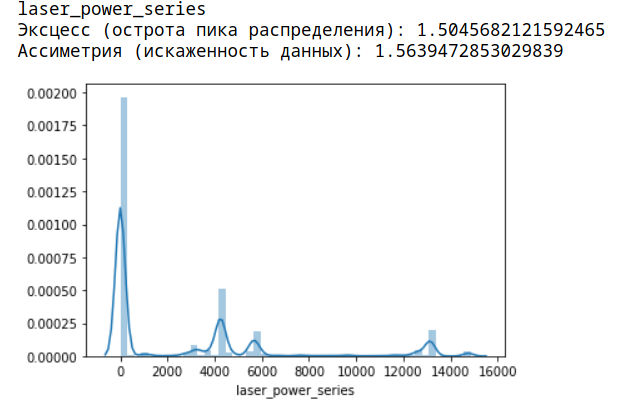
\includegraphics[width=13cm]{powerstruct.png}}
    \caption{Проверка структуры распределения мощности лазера}
    \label{powerstruct}
\end{figure}

На рисунках \ref{tempstruct} и \ref{powerstruct} отображены данные по структуре распределений
температуры и мощности лазера.
Видно, что структура у обоих распределений комплексная,
состоящая из смеси распределений с нетривиальными свойствами.

\newpage

\subsubsection{Анализ трендов}

На рисунке \ref{trends} видно, что данные в основном
имеют устойчивый тренд по месяцам.
Дисперсия данных температуры лазера невысокая.

\begin{figure}[H]
    \center{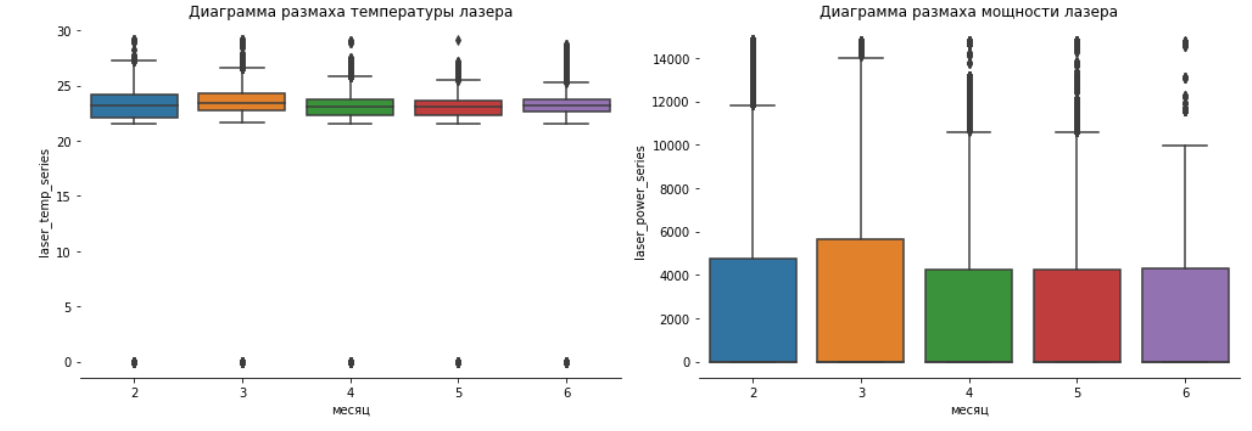
\includegraphics[width=15cm]{trends.png}}
    \caption{Диаграммы размаха}
    \label{trends}
\end{figure}

На рисунках \ref{tempdiv} и \ref{powerdiv} отображены
тренды по дням, неделям и месяцам.
Заметно, что тренд мощности лазера уменьшается.
Это говорит о том, что лазерная голова
станка начинает изнашиваться,
поэтому данный тренд необходимо отслеживать.

\begin{figure}[H]
    \center{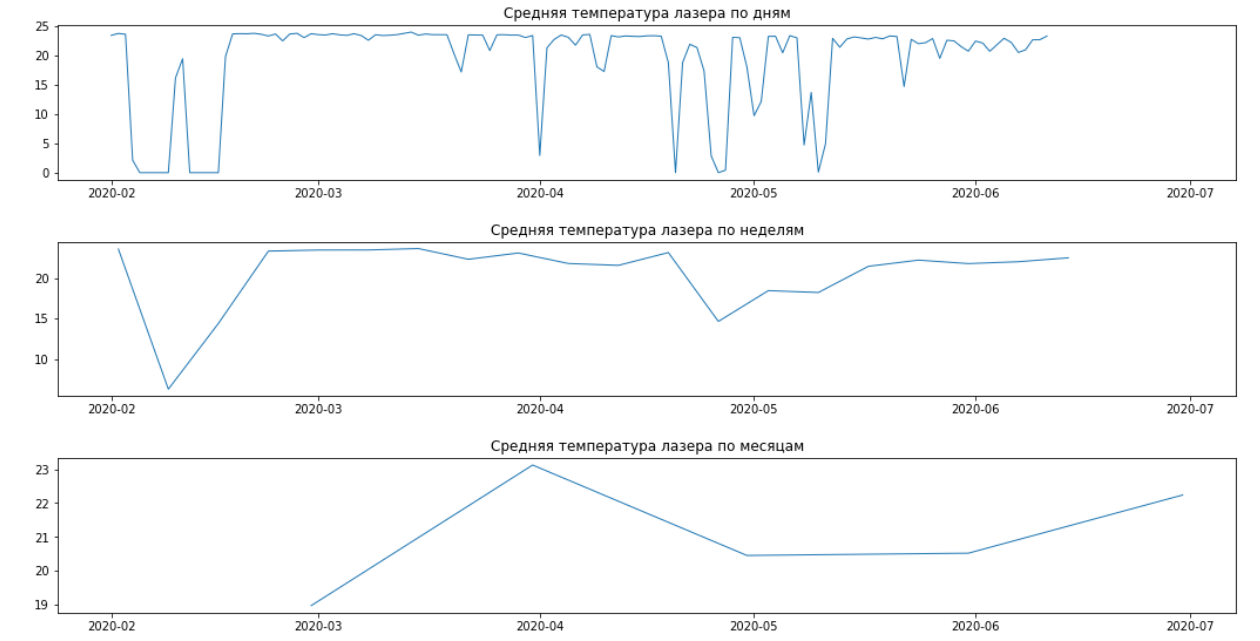
\includegraphics[width=15cm]{tempdiv.png}}
    \caption{Тренды температуры лазера}
    \label{tempdiv}
\end{figure}

\begin{figure}[H]
    \center{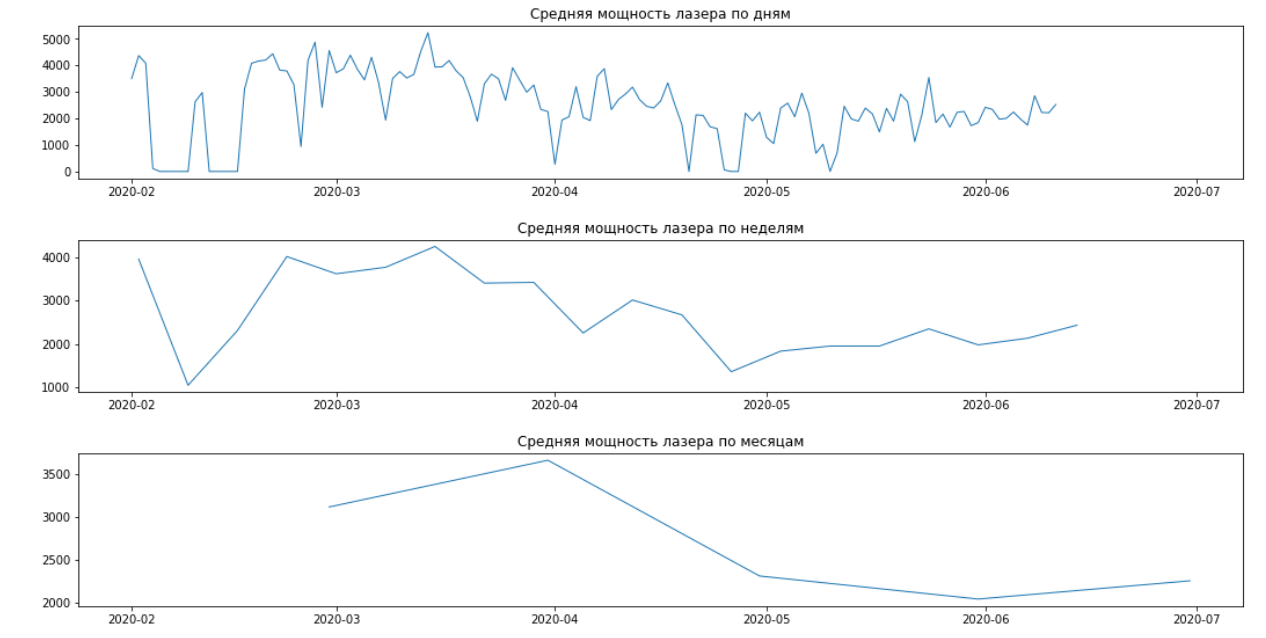
\includegraphics[width=15cm]{powerdiv.png}}
    \caption{Тренды мощности лазера}
    \label{powerdiv}
\end{figure}


На риунке \ref{checkpower} отображены временные
ряды за короткие период двух параметров: фактическая и установленная мощность.
Видно, что установленная мощность постоянна, однако ее могут изменять.
Инженеры компании ВНИТЭП также рекомендуют следить
за регулярным превышением фактической мощности,
что может привести к более быстрому износу,
однако, как уже было описано,
тренд мощности пока только падает.
Для системы предупреждения важно обозначить требования,
на основе которых позволялось использовать мощность
лазера выше установленной в течение какого-то интервала времени.


\begin{figure}[H]
    \center{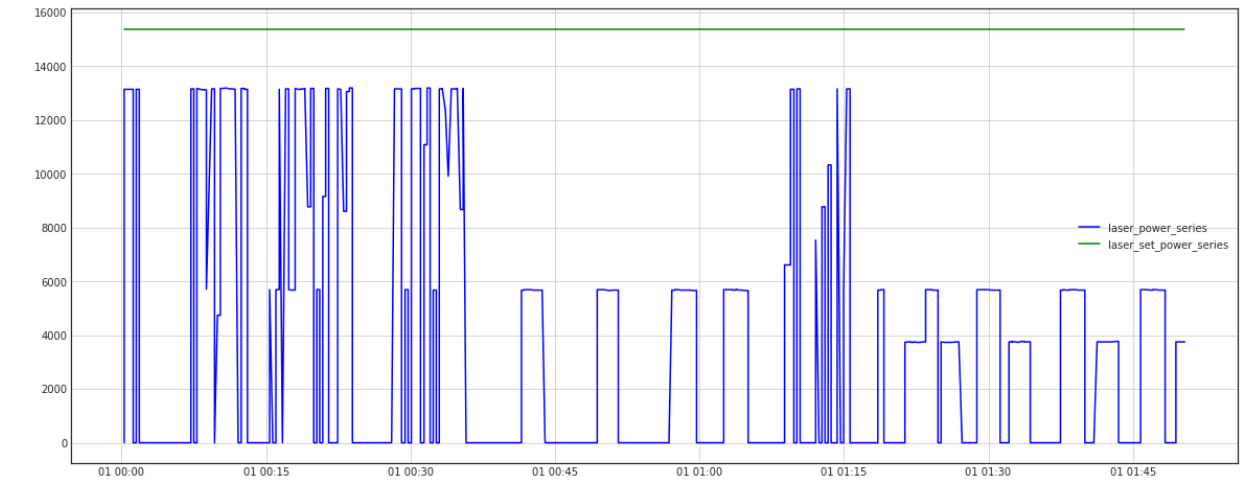
\includegraphics[width=15cm]{checkpower.png}}
    \caption{Фактическая и установленная мощность}
    \label{checkpower}
\end{figure}


Рисунок \ref{powertemp} представляет собой отображение
очевидной связи между мощностью и температурой лазера.
Данные на рисунке нормализованы для наглядного сравнения.

\begin{figure}[H]
    \center{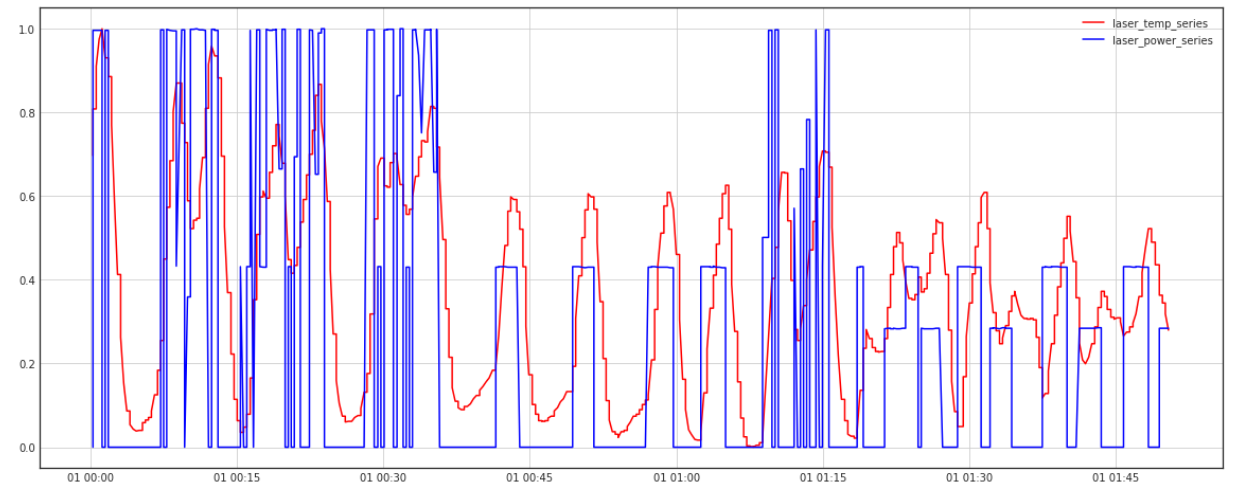
\includegraphics[width=15cm]{powertemp.png}}
    \caption{Отношение температуры и мощности лазера}
    \label{powertemp}
\end{figure}


\subsubsection{Тестирование на стационарность}

Для того, чтобы всецело использовать дальнейшие более сложные методы,
необходимо узнать являются ли исследуемые
временные ряды стационарными.
Именно стационарность позволяет
более эффективно работать с временными рядами.
Для этого можно использовать тест Дики-Фуллера.
Данный тест позволяет определить меру того,
насколько данный временной ряд является стационарным.

\begin{figure}[H]
    \center{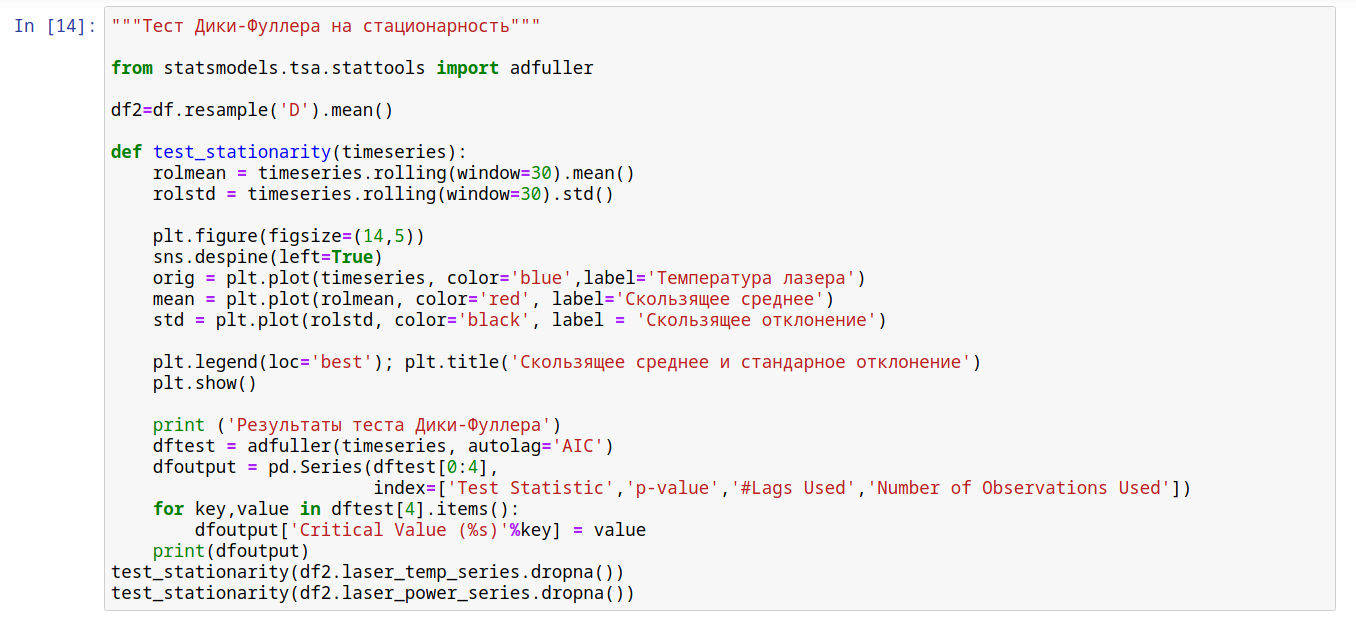
\includegraphics[width=16.5cm]{fuller.png}}
    \caption{Код для теста Дики-Фуллера}
    \label{fuller}
\end{figure}

На рисунке \ref{fuller} отображен код,
в котором анализируются два временных ряда температуры и мощности лазера на стационарность.
Оба ряда усреднены по дням.

\begin{figure}[H]
    \center{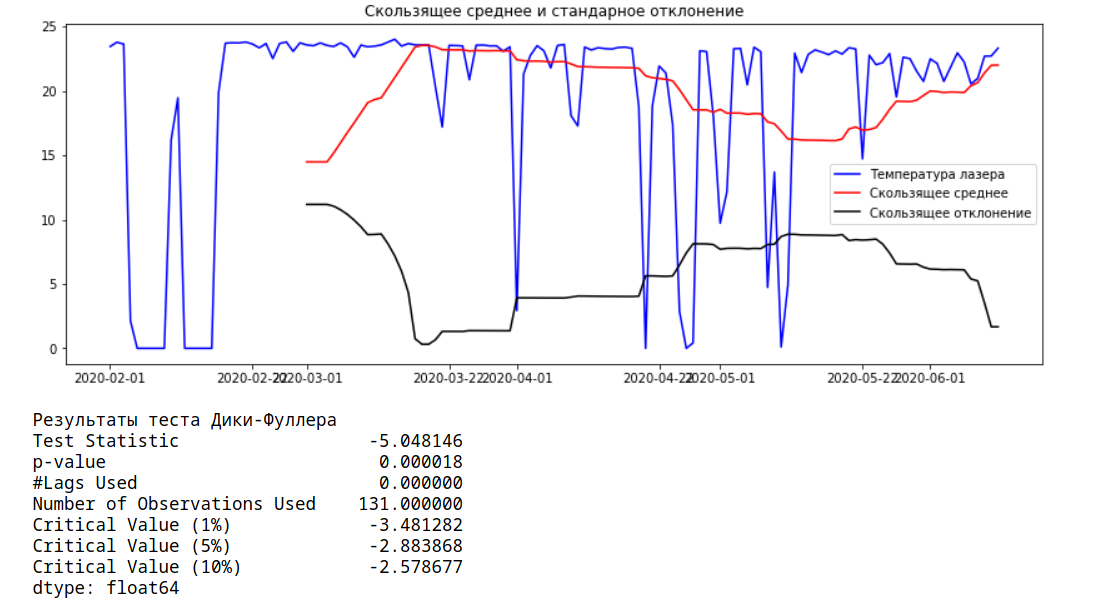
\includegraphics[width=15cm]{fullertemp.png}}
    \caption{Результаты теста для температуры лазера}
    \label{fullertemp}
\end{figure}

\begin{figure}[H]
    \center{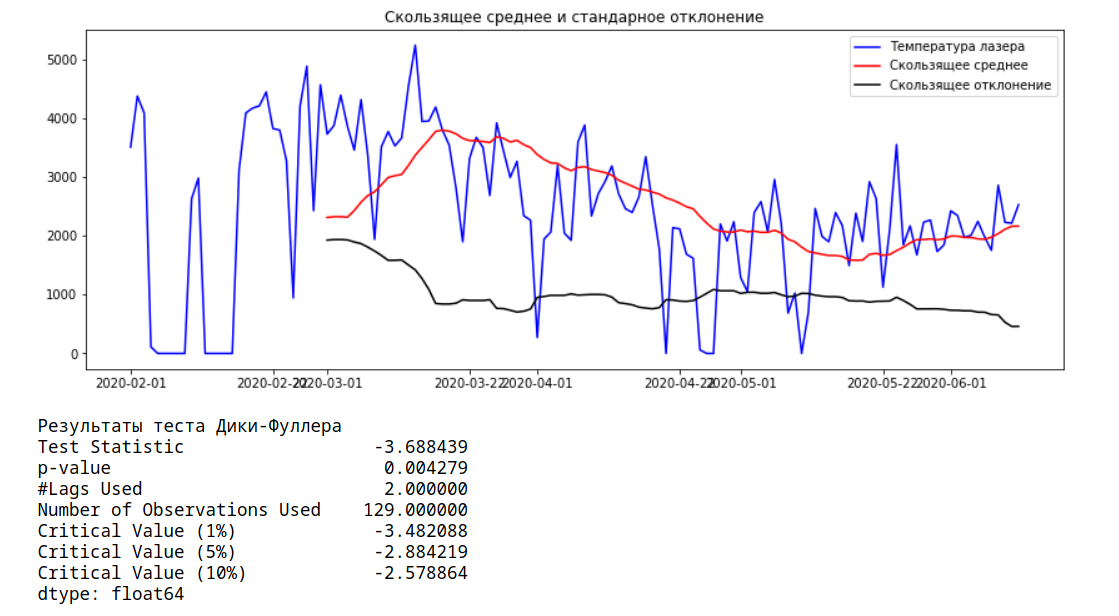
\includegraphics[width=15cm]{fullerpower.png}}
    \caption{Результаты теста для мощности лазера}
    \label{fullerpower}
\end{figure}

На рисунках \ref{fullertemp} и \ref{fullerpower} отображен результат
выполнения теста с дополнительными параметрами.
Основным условием для принятия гипотезы стационарности
было p-значения меньше $0,05$,
что означает то,
что у ряда нет единичных корней 
(характеристическое уравнение авторегрессионной модели временного ряда не имеет корней равных по модулю единице).
Как видно из рисунков, ряды проявляют свойства стационарности.


\subsection{Архитектура разработанного решения}

На рисунке \ref{pipeline} отображена архитектура
в виде однонаправленного графа,
узлы которых являются модулями разработанного решения,
а вершины -- поток данных.
Поток разбивается на два параллельных
процесса вычислений: предсказание и генерацию признаков.

\begin{figure}[H]
    \center{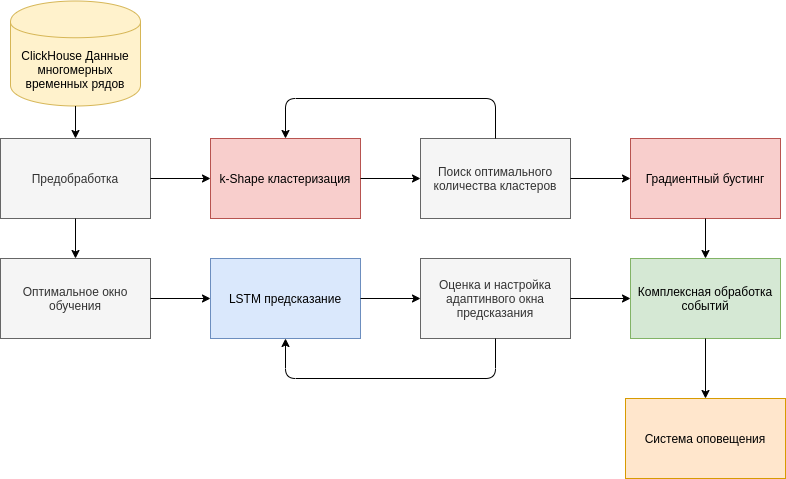
\includegraphics[width=15cm]{pipeline.png}}
    \caption{Диаграмма архитектуры}
    \label{pipeline}
\end{figure}

За предсказание отвечает нейронная сеть LSTM архитектуры,
с дополнительными особенностями в виде определения
оптимального окна обучения для повышения точности
и адаптивного окна предсказания,
также для повышения точности.

Алгоритмы k-Shape и градиентный бустинг
отвечают за выявление дополнительных признаков,
характеризующих набор данных.
Данный подход необходим для выявления
дополнительных паттернов,
некоторые из которых могут быть признаками неисправностей,
либо близких к неисправностям состояний.
Возможно, что данный блок может не помочь
в поиске неисправностей, однако такой блок поспособствует лучшему понимаю данных.

Предсказанные LSTM данные и модель градиентного бустинга
объединяют в модули комплексной обработки событий.
Моделью градиентного бустинга и некоторыми
наложенными условиями определяется
являются ли предсказанные отрезки времени
потенциальными неисправностями или сбоями,
либо нормальным состоянием.
В случае выявления неисправностей,
в зависимости от рода неисправностей,
происходит обработка результатов и
конечные данные отправляются в систему оповещения о неисправностях.

Поток данных может обрабатываться рекуррентно в блоках
предсказания и кластеризации с целью повышения точности.

\subsection{Обучение LSTM}

Обучение моделей на временных рядах может происходить различными способами.
Основным способ является обучение на основе скользящего окна.
Предположим, что есть временной ряд $TS = \{x_1, ..., x_n\}$.
Тогда, скользящим окном называется фрагмент ряда $TS$ размера $m$ с шагом $s$.
Тем самым, исходный ряд разбивается на сегменты одинакового размера: $TS = \{S_1, ..., S_{\frac{n}{s}}\}$.
В данной работе оптимальный размер окна вычисляется на основе периодограмма
построенной с помощью метода Ломба-Скаргл, который был описан в предыдущем разделе.
Также стоит отметить, что общее окно обучения,
то есть отрезок всего временного ряда выбран максимальным,
так как нейронные сети лучше обучаются на большем количестве данных.

\begin{figure}[H]
    \center{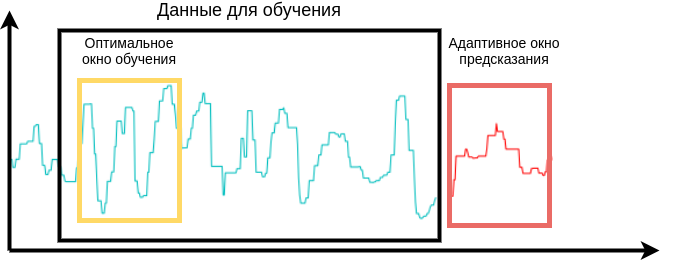
\includegraphics[width=15cm]{windows.png}}
    \caption{Описание различных окон временного ряда}
    \label{windows}
\end{figure}

На рисунке \ref{windows} описано примерное представление различных окон,
которые могут настраиваться на основе тех или иных критериев оптимальности.
На диаграмме также присутствует так называемое
адаптивное окно предсказания, которое определяется
на основе наиболее меньшего значения функции потерь.

\begin{figure}[H]
    \center{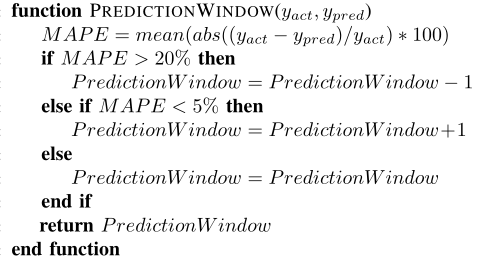
\includegraphics[width=13cm]{predwindow.png}}
    \caption{Алгоритм адаптивного окна предсказания}
    \label{predwindow}
\end{figure}

\begin{equation} \label{mape}
    MAPE = \frac{1}{n} \sum_{t=1}^n \Big| \frac{A_t - F_t}{A_t} \Big|
\end{equation}

На рисунке \ref{predwindow} описан псевдокод программы для вычисления адаптивного окна предсказания.
MAPE (mean absolute percentage error) -- средняя абсолютная процентная ошибка,
являющейся мерой точности предсказания и выражается по формуле \ref{mape},
$A_t$ -- реальное значение, а $F_t$ -- предсказанное.

\begin{figure}[H]
    \center{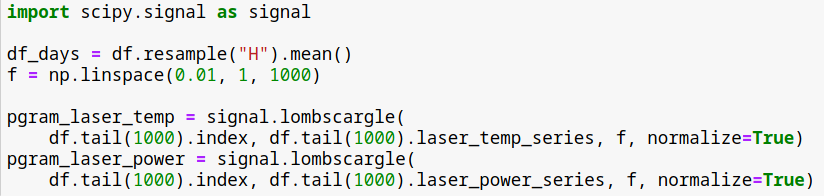
\includegraphics[width=13cm]{optimalcode.png}}
    \caption{Код для использования метода Ломба-Скаргл}
    \label{optimalcode}
\end{figure}

В программном коде на рисунке \ref{optimalcode}  происходит
вычисление периодограмм для усредненных по часам временных рядов
температуры и мощности лазера. Для этого использовалась библиотека Scipy.
Данные автоматически нормализуются и на основе заданной частоты определяются преобладающие частоты временных рядов.

\begin{figure}[H]
    \center{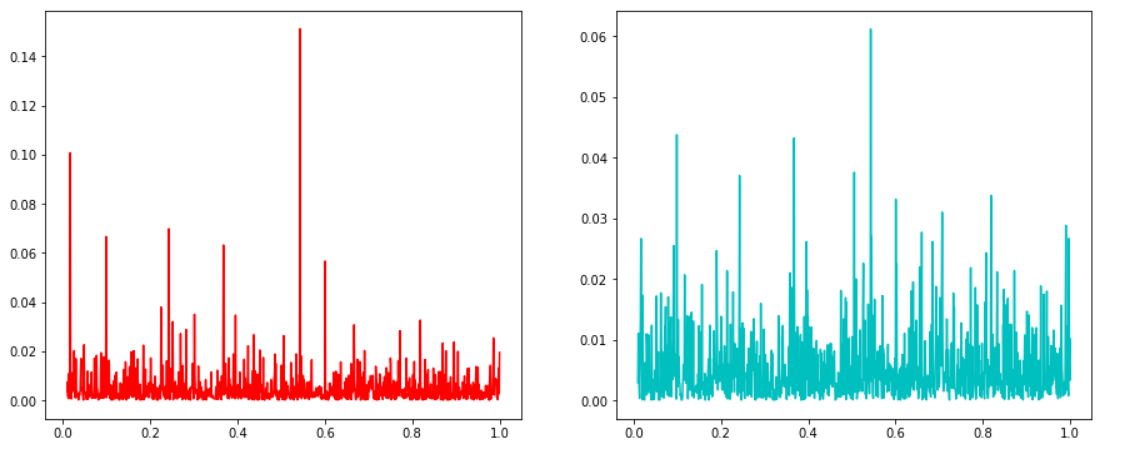
\includegraphics[width=13cm]{optimal.png}}
    \caption{Результат использования метода Ломба-Скаргл}
    \label{optimal}
\end{figure}

На рисунке \ref{optimal} видно, что сильно выделенных частот в данных почти нет,
однако в обоих случаях преобладают частоты около значения 0.5, поэтому
можно сказать, что оптимальным историческим окном обучения является разбиение данных на последнюю половину.

\begin{figure}[H]
    \center{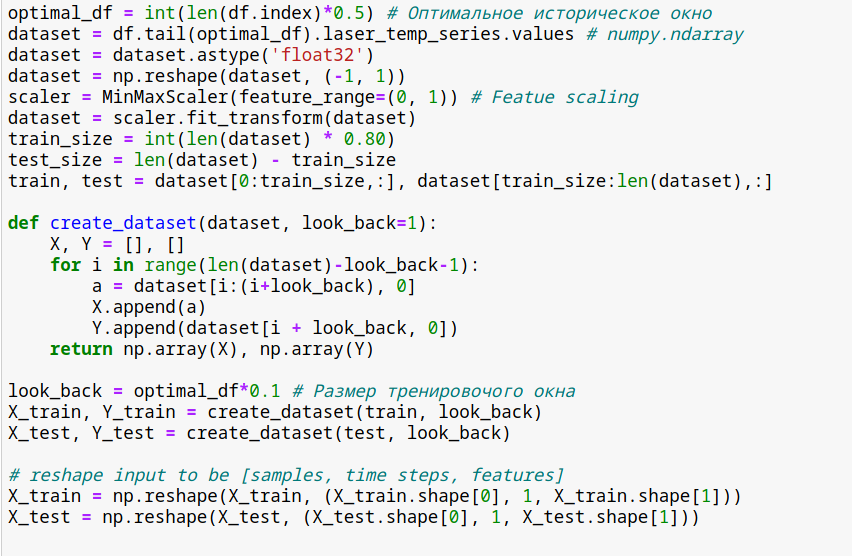
\includegraphics[width=16cm]{preptemp.png}}
    \caption{Подготовка выборок температуры лазера для обучения LSTM}
    \label{preptemp}
\end{figure}

На рисунке \ref{preptemp} отображен код для подготовки данных для тренировки.
В данном случае описан код с разбиением выборок на тренировочную и тестовую
в соответствии с выделенными оптимальными окнами в виде $\{(\textbf{x}_i,y_i)\}_{i=1}^n$.
В последующем данный код будет встраиваться и динамически
изменять параметры оптимальных окон обучения и предсказания
на основе описанных методов.
 
\begin{figure}[H]
    \center{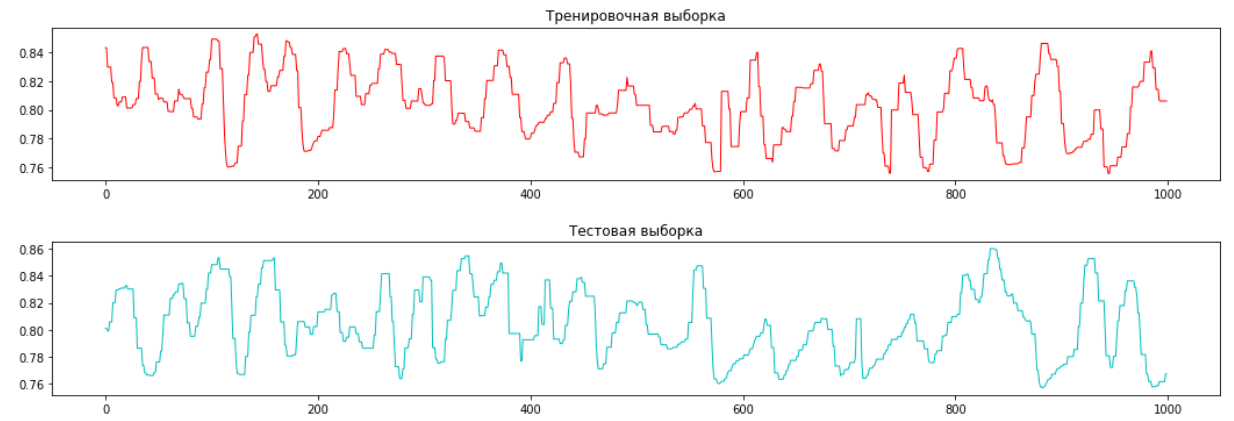
\includegraphics[width=15cm]{samptemp.png}}
    \caption{Подготовленные выборки температуры лазера}
    \label{samptemp}
\end{figure}

\begin{figure}[H]
    \center{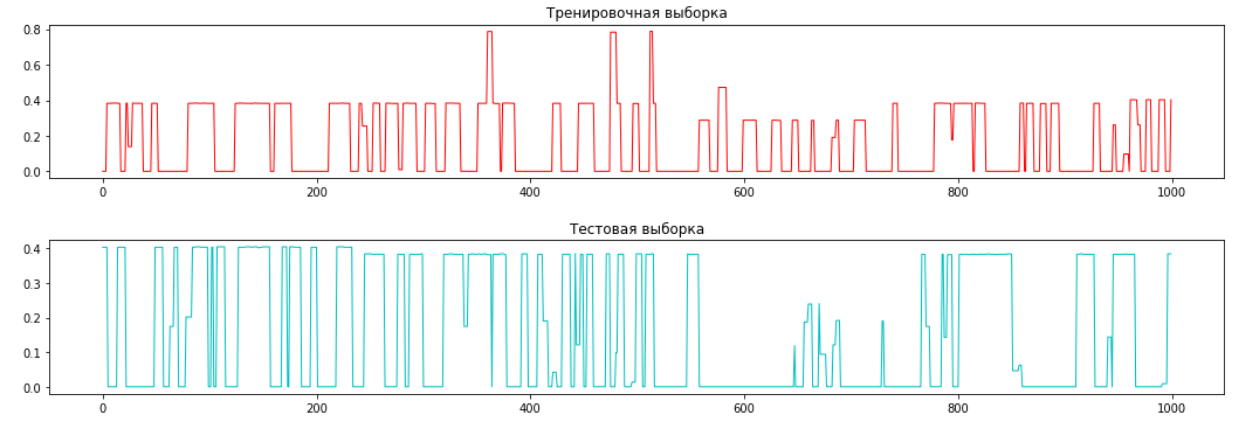
\includegraphics[width=15cm]{sampwer.png}}
    \caption{Подготовленные выборки мощности лазера}
    \label{sampwer}
\end{figure}

На графиках рисунков \ref{samptemp} и \ref{sampwer} отображены
первые 1000 значений тренировочных и тестовых выборок.


\begin{figure}[H]
    \center{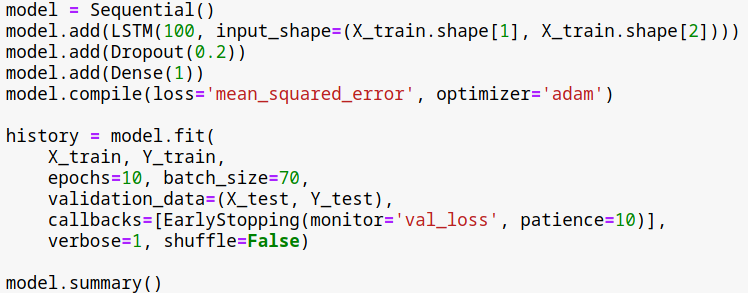
\includegraphics[width=15cm]{lstmfit.png}}
    \caption{Код для тренировки нейронной сети LSTM}
    \label{lstmfit}
\end{figure}

Для тренировки нейронной сети LSTM был выбран ряд параметров (рисунок \ref{lstmfit}).
Для самой сети было определено 100 нейронов. Такой показатель не обязательно является оптимальным,
но может быть достаточно подходящим для большинства случаев.

Кроме этого, для тренировки используется метод регуляризации Dropout,
который представляет собой случайное исключение определенного процента нейронов
в процессе обучения нейронной сети.
Данный метод нацелен на предотвращение переобучения сети,
и, эмпирически, было выведено то, что такой вид регуляризации наиболее эффективен
для большинства случаев.
Для разрабатываемой системы был выбран Dropout в размере 20 процентов,
что также как и количество нейронном не обязательно является оптимальным,
однако является вполне подходящим вариантом.

Была выбрана функция потерь в виде среднеквадратичной ошибки,
а также метод для стохастической оптимизации этой функции Adam.
Метод Adam считается наилучшим для оптимизации функций потерь
на 2020 год.
Для поиска оптимального окна будет использоваться другая функция потерь,
как уже было описано, а именно средняя абсолютная процентная ошибка.

Для тренировки был выбран размер отправляемых данных,
который равен 70, а также количество тренировочных эпох равным 10,
что является достаточным.

\begin{figure}[H]
    \center{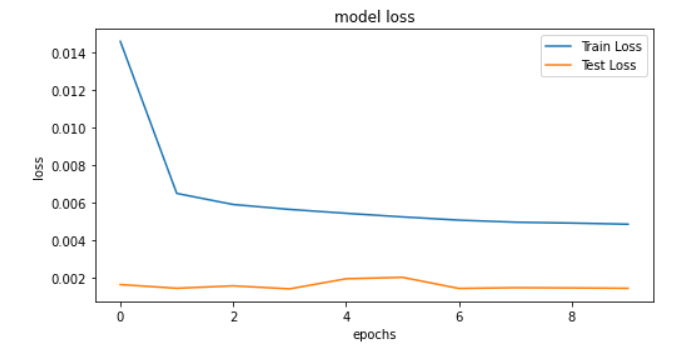
\includegraphics[width=13cm]{losstemp.png}}
    \caption{Динамика функций потерь в процессе тренировки LSTM для температуры лазера}
    \label{losstemp}
\end{figure}

\begin{figure}[H]
    \center{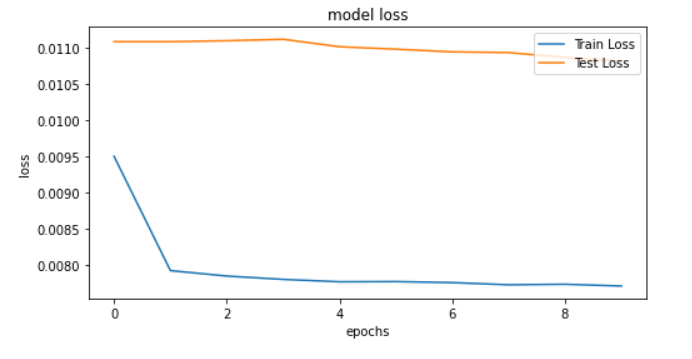
\includegraphics[width=13cm]{losspower.png}}
    \caption{Динамика функций потерь в процессе тренировки LSTM для мощности лазера}
    \label{losspower}
\end{figure}


Графики на рисунках \ref{losstemp} и \ref{losspower}
отображают динамику изменения значений функций потерь (loss)
на тренировочной и тестовых выборках
в процессе тренировки по эпохам (epochs).
Для данных температуры лазера
минимизация прошла успешнее,
чем для данных мощности лазера.


\begin{figure}[H]
    \center{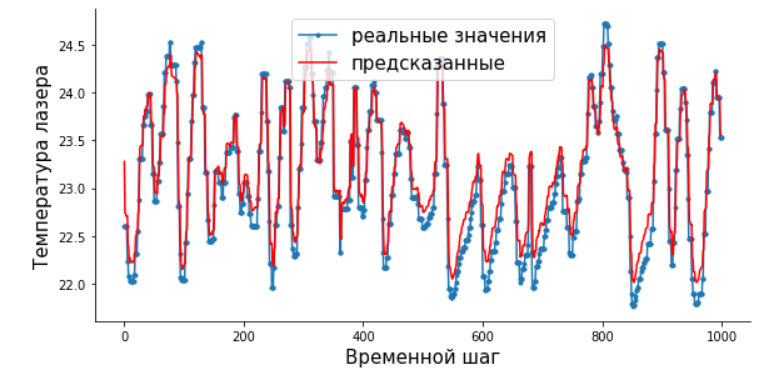
\includegraphics[width=15cm]{predtemp.png}}
    \caption{Реальные и предсказанные значения для температуры лазера}
    \label{predtemp}
\end{figure}


\begin{figure}[H]
    \center{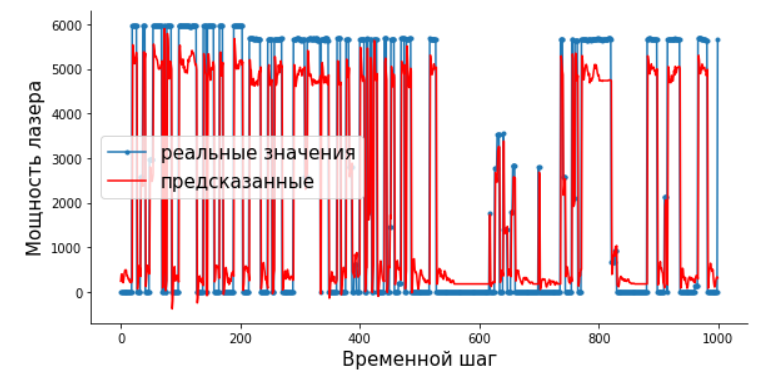
\includegraphics[width=15cm]{predpower.png}}
    \caption{Реальные и предсказанные значения для мощности лазера}
    \label{predpower}
\end{figure}

Итоговые результаты предсказания значений отображены
на графиков рисунков \ref{predtemp} и \ref{predpower}
для первых 1000 значений.
Предсказанные значения для температур
оказались лучше, чем для мощности.
Такой результат получился по причине
нетривиальной структуры временных рядов мощности лазера.
Однако, такая разница не является критичной,
так как температура зависит от мощности,
что означает возможность использования только температурных значений.

\subsection{Кластеризация на основе k-Shape}


Кластеризация является экспериментальным этапом в процессе обработки данных станка лазерной резки
и может быть иметь неопределенные результаты.
Однако, в данной работе описаны первоначальные результаты использования алгоритма k-Shape,
которые будут в дальнейшем улучшаться за счет использования оптимизационных методов.

Многие алгоритмы кластеризации
требуют предварительную установку количества кластеров.
Такая задача является исследовательской
и полноценно пока не решена.
Обычно, выбор количества кластеров
зависит от специфики задачи.
В задаче распознавания неисправностей сложно
определить подходящее количество кластеров
без использования автоматических оптимизационных методов.
Однако, было определено 3 кластера: для нормального состояния,
для среднего и для состояния неисправности.


На рисунке \ref{kshapecode} отображен код для подготовки данных температуры лазера,
использования алгоритма k-Shape на основе Tslearn и вывода результатов
при помощи библиотеки Matplotlib.
Было выбрано окно длинной 10 с шагом в половину тренировочного исторического окна.
Кроме этого, данные были нормализованы на основе z-нормализации при помощи
функции $TimeSeriesScalerMeanVariance()$.

На рисунке \ref{kshaperes} отображен результат кластеризации временного ряда
температуры лазера. По данным результатам видно, что выявлены
три паттерна-состояния станка: снижение, повышение и стабильное состояние.
На основе выявленных паттернов можно создать модель классификации
для предсказанных данных, что и будет использовано для градиентного бустинга
в дальнейшем.

\begin{figure}[H]
    \center{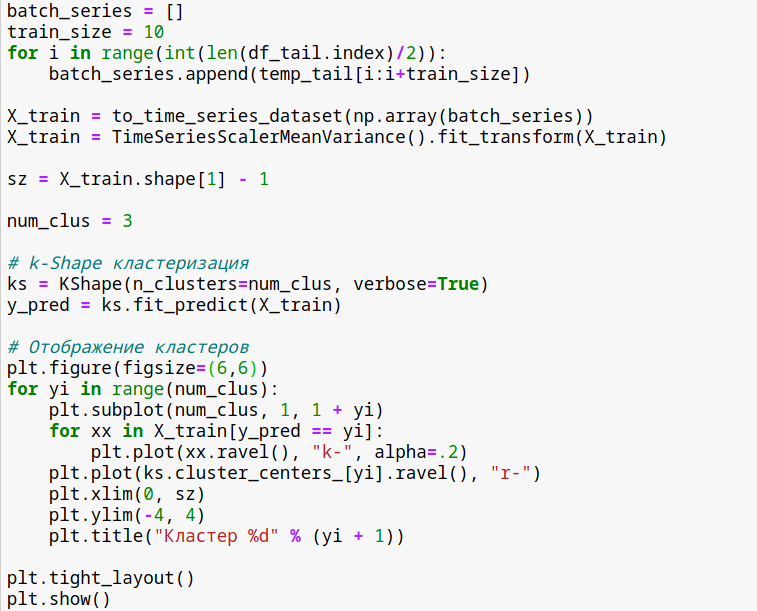
\includegraphics[width=13cm]{kshapecode.png}}
    \caption{Код для использования алгоритма k-Shape}
    \label{kshapecode}
\end{figure}

\begin{figure}[H]
    \center{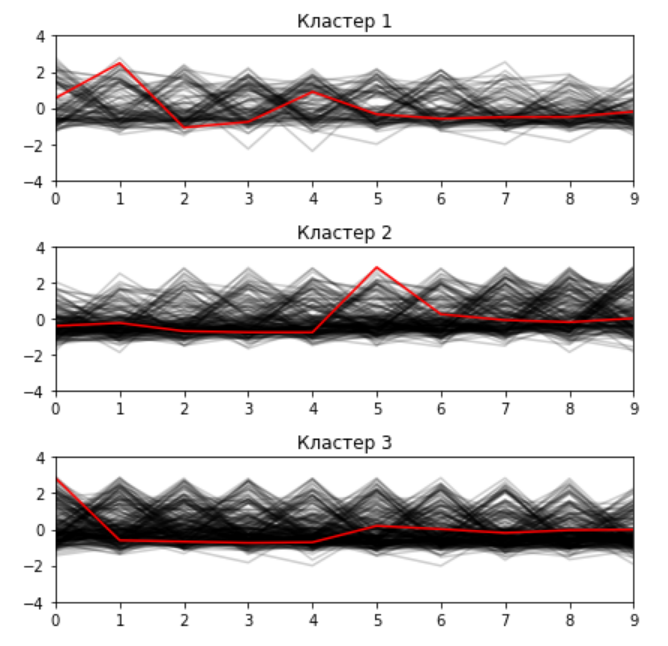
\includegraphics[width=11cm]{kshaperes.png}}
    \caption{Результаты кластеризации}
    \label{kshaperes}
\end{figure}

\subsection{Анализ предсказанных значений}

Предсказанные на основе LSTM
временные ряды могут использоваться для
последующей проверки на выявление неисправностей.
Для определения неисправностей используется
анализ трендов и среднего предсказанных значений.

Критичным для значения температуры
является стойкая высокая температура выше 120 градусов,
и стойкая низкая температура ниже 30 градусов по Цельсию,
на протяжении длительного времени (около суток).
Для мощности лазера необходимо отслеживать
тренд ее снижения на протяжении суток, а также превышение используемой мощности выше заданной в течение минуты.
Данные ограничения для исследуемых параметров станка Навигатор
определены на основе инженерных требований разработчиков станка компании ВНИТЭП.

Описанные ограничения будут реализованы
в мироксервисе Omniprocessing на основе простого подсчета
среднего с использованием микросервиса статистики Gorobots,
а также на основе простых условных конструкций,
написанных на языке Python.

\subsection{Введение в эксплуатацию}

Вся описанная архитектура разработанного модуля
для предсказания и определения неисправностей будет интегрирована,
как уже было описано, в микросервис Omniprocessing.
Однако, необходимо решить ряд проблем,
связанных с кластеризацией и использованием алгоритма градиентного бустинга,
а именно определение оптимальных параметров для алгоритмов,
например, определение оптимального количества кластеров.
Сам алгоритм градиентного бустинга необходимо реализовывать на основе оптимизированной кластеризации,
поэтому в данной работе он не был описан.
Кроме этого, сама интеграция является нетривиальной задачи
и требует решения проблем связанных с сопряжением всех подмодулей
с учетом среды, в которой эти подмодули интегрируются,
а именно в среде фреймворка Faust.
Также отдельной задачей является использование сервиса Gorobots
для подсчета средних трендов и предсказанных значений.

После решения поставленных задач,
разработанный модуль будет разворачиваться
вместе со всей платформой компании Omnicube
с использованием Kubernetes.
Отчет о неисправностях будет отправлен
в сервис оповещения OmniNotifier.

\subsection{Выводы}

На основе предобработки данных со станка лазерной резки Навигатор КС-12В
был проведен первичный анализ особенностей и свойств выделенных параметров станка:
температуры и мощности лазера.
Для этого был проведен ряд тестов: на нормальность и на стационарность рядов.

Выявлено оптимальное окно для тренировки модели предсказания.
Описано использование модели предсказания -- нейронной сети LSTM.
Дана характеристика гиперпараметров модели.

Описано использование алгоритма k-Shape для кластеризации,
а также результаты этого использования.
Выявлены паттерны состояний станка, который могут
в дальнейшем будут использоваться алгоритмом градиентного бустинга.
Обозначены проблемы оптимизации данного алгоритма.

В конце раздела дано описание принципов интеграции с системой компании Omnicube.

\clearpage